\documentclass[10pt, aspectratio=169]{beamer}

\usepackage[T1]{fontenc}
\usepackage[utf8]{inputenc}
\usepackage[english]{babel}
\usepackage{lmodern}
\usepackage{amsmath, amssymb}
\usepackage{booktabs}
\usepackage{array}
\usepackage{tikz}
\usetikzlibrary{arrows.meta}

% Same drawing styles as the report (FINAL/report/main.tex)
\tikzset{
  agent/.style    = {circle, draw, inner sep=0pt, minimum size=4.5mm, font=\scriptsize},
  edge/.style     = {-{Stealth[length=1.6mm]}, thin},
  selfloop/.style = {-{Stealth[length=1.6mm]}, thin, loop above, looseness=6, min distance=4mm},
  weight/.style   = {font=\tiny, inner sep=1pt}
}

% Figures are taken directly from the report
\graphicspath{{../report/figures/}}

% Use Unipd as theme, with options:
% - pageofpages: define the separation symbol of the footer page of pages (e.g.: of, di, /, default: of)
% - logo: position another logo near the Unipd logo in the title page (e.g. department logo), passing the second logo path as option
% Use the environment lastframe to add the endframe text
\usetheme[pageofpages=of]{Unipd}

\title[Stubbornness and social power in opinion dynamics]{Stubbornness and Social Power\\ in Opinion Dynamics}
\subtitle{The French--Harary--DeGroot and Friedkin--Johnsen models}
\author[Leonardo Luigi Pepe]{Leonardo Luigi Pepe}
\date{Network Dynamical Systems, A.Y.\ 2025/26 \\ 26 November 2026}

% ---------------------------------------------------------------------------
% Links between the main slides and the backup slides (appendix)
%   \detailbuttons{...} puts buttons in the bottom-right corner of a slide
%   \go{label}{text}    button to a backup slide
%   \ret[text]{label}   button back to a main slide
% ---------------------------------------------------------------------------
\newcommand{\detailbuttons}[1]{%
  \begin{tikzpicture}[remember picture, overlay]
    \node[anchor=south east, inner sep=0pt] at ([xshift=-3mm, yshift=6mm]current page.south east) {#1};
  \end{tikzpicture}}
\newcommand{\go}[2]{\hyperlink{#1}{\beamergotobutton{#2}}}
\newcommand{\ret}[2][Back]{\hyperlink{#2}{\beamerreturnbutton{#1}}}

% Reading in social terms: a green block that leaves room for the buttons on the right
\newcommand{\socially}[1]{%
  \begin{minipage}{0.76\textwidth}
    \begin{exampleblock}{In social terms}\footnotesize #1\end{exampleblock}
  \end{minipage}}

\newcommand{\sociallycol}[1]{%
  \begin{exampleblock}{In social terms}\footnotesize #1\end{exampleblock}}

% Colour code of the blocks
%   block        (blue)  : statements from the sources, as in the report
%   exampleblock (green) : reading in social terms
%   alertblock   (red)   : key message

\begin{document}

% Make the title page
\frame{\titlepage}

\begin{frame}{Outline}
  \tableofcontents
\end{frame}

% ===========================================================================
\section{Introduction}
% ===========================================================================

\begin{frame}[label=m-question]{Stubbornness}
  \begin{itemize}
    \item A social network is a weighted digraph: agents are nodes, edges carry the
          influence, opinions are updated by repeated averaging.
    \item A \alert{stubborn} agent never changes its opinion [5]. It is the extreme case of
          two graded mechanisms of resistance:
          \begin{itemize}
            \item FDG model: a \alert{self-weight} $a_{ii}$ on the \emph{current} opinion
                  \hfill $\to$ inertia
            \item FJ model: an \alert{attachment} $1-\lambda_i$ to a \emph{fixed} prejudice
                  $u_i$ \hfill $\to$ anchor
          \end{itemize}
  \end{itemize}
  \vspace{3mm}
  \begin{alertblock}{Three questions, asked of both models on the same networks}
    \begin{enumerate}
      \item Do the opinions converge?
      \item What do they converge to?
      \item How much does each agent weigh? \quad social power $w$ (FDG), influence
            centrality $c$ (FJ)
    \end{enumerate}
  \end{alertblock}
\end{frame}

\begin{frame}[label=m-models]{Models of opinion dynamics}
  \centering
  \begin{tikzpicture}[
      box/.style  = {draw, rounded corners=2pt, align=center, font=\footnotesize,
                     text width=4.1cm, minimum height=1.25cm, inner sep=3pt},
      sel/.style  = {box, very thick, draw=red_unipd, fill=red_unipd!7},
      oth/.style  = {box, draw=gray, text=gray!70!black},
      lab/.style  = {font=\footnotesize\bfseries, align=center},
      arr/.style  = {-{Stealth[length=2mm]}, thick}]
    \node[lab] at (0, 1.25) {consensus models};
    \node[lab] at (5.6, 1.25) {with prejudices};
    \node[lab, anchor=east] at (-2.45, 0) {discrete\\ time};
    \node[lab, anchor=east] at (-2.45, -1.6) {continuous\\ time};
    \node[sel] (fdg) at (0, 0) {\textbf{French--Harary--DeGroot}\\
      French 1956, Harary 1959--65,\\ DeGroot 1974};
    \node[sel] (fj) at (5.6, 0) {\textbf{Friedkin--Johnsen}\\
      1990s, validated on small\\ and medium-size groups};
    \node[oth] (ab) at (0, -1.6) {\textbf{Abelson} 1964\\ consensus too strong:\\
      the cleavage problem};
    \node[oth] (ta) at (5.6, -1.6) {\textbf{Taylor} 1968\\ constant external opinions};
    \draw[arr, red_unipd] (fdg) -- node[above, font=\scriptsize] {+ prejudices} (fj);
    \draw[arr, gray] (ab) -- node[above, font=\scriptsize] {+ prejudices} (ta);
  \end{tikzpicture}

  \vspace{4mm}
  \raggedright
  \small
  \begin{itemize}
    \item Historical account of the tutorial by Proskurnikov and Tempo [5], the main source,
          with the course slides [1--3] and the book by Bullo [4].
    \item This work: the \alert{FDG model} (seen in the course) and the \alert{FJ model}
          (new). Abelson and Taylor only as an overview.
  \end{itemize}
\end{frame}

\begin{frame}[label=m-networks]{Two networks, one agent}
  \begin{columns}[T]
    \column{0.46\textwidth}
      \centering
      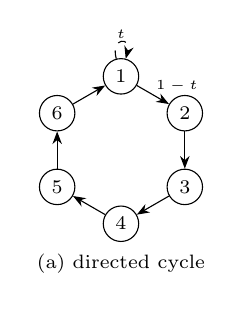
\begin{tikzpicture}[baseline=(c.base), scale=0.72]
        \foreach \i in {1,...,6} {
          \node[agent] (d\i) at ({90-60*(\i-1)}:1.3) {\i};
        }
        \node (c) at (0,0) {};
        \foreach \i/\j in {2/3,3/4,4/5,5/6,6/1} {
          \draw[edge] (d\i) -- (d\j);
        }
        \draw[edge] (d1) -- node[weight, above right] {$1-t$} (d2);
        \draw[selfloop, dashed] (d1) to node[weight, above] {$t$} (d1);
        \node at (0,-2.0) {\scriptsize (a) directed cycle};
      \end{tikzpicture}
      \hspace{1mm}
      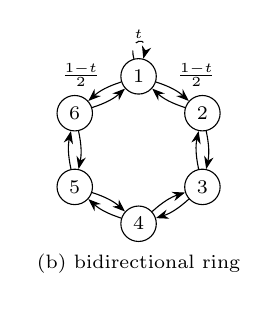
\begin{tikzpicture}[baseline=(c.base), scale=0.72]
        \foreach \i in {1,...,6} {
          \node[agent] (b\i) at ({90-60*(\i-1)}:1.3) {\i};
        }
        \node (c) at (0,0) {};
        \foreach \i/\j in {2/3,3/4,4/5,5/6} {
          \draw[edge] (b\i) to[bend left=12] (b\j);
          \draw[edge] (b\j) to[bend left=12] (b\i);
        }
        \draw[edge] (b2) to[bend left=12] (b1);
        \draw[edge] (b6) to[bend right=12] (b1);
        \draw[edge] (b1) to[bend left=12] node[weight, above right] {$\frac{1-t}{2}$} (b2);
        \draw[edge] (b1) to[bend right=12] node[weight, above left] {$\frac{1-t}{2}$} (b6);
        \draw[selfloop, dashed] (b1) to node[weight, above] {$t$} (b1);
        \node at (0,-2.0) {\scriptsize (b) bidirectional ring};
      \end{tikzpicture}

      \vspace{2mm}
      {\scriptsize Figure 1. Edge $i \to j$: agent $i$ is influenced by agent $j$\\
      (course convention).}
    \column{0.52\textwidth}
      \small
      \begin{itemize}
        \item $n = 6$. Cycle: $a_{i,i+1} = 1$. Ring: $a_{i,i\pm1} = 1/2$.
        \item Strongly connected and \alert{periodic} (period $6$ and $2$), doubly
              stochastic: $w = \frac16\mathbf{1}_6$, no agent favoured.
        \item Only agent~$1$ changes, with self-weight $t$:
              \[ a_1(t)^\top = (1-t)\, a_1^\top + t\, e_1^\top \;\to\; A(t), \]
              from the original network ($t = 0$) to agent~$1$ stubborn ($t = 1$).
        \item Always $x(0) = (0,\, 0.2,\, 0.4,\, 0.6,\, 0.8,\, 1)^\top$.
      \end{itemize}
  \end{columns}
\end{frame}

% ===========================================================================
\section{The French--Harary--DeGroot model}
% ===========================================================================

\begin{frame}[label=m-fdg-model]{The FDG model}
  \begin{columns}[T]
    \column{0.40\textwidth}
      \small
      \[ x(k+1) = A\, x(k), \quad A \geq 0,\; A\mathbf{1}_n = \mathbf{1}_n \]
      \begin{itemize}
        \item Each agent takes a weighted average of the opinions it listens to: a DT
              averaging system [1].
        \item $x(k) = A^k x(0)$: the spectrum of $A$ decides; the eigenvalue $1$ is
              always there (Theorem~1.6).
        \item Three outcomes (Definition~2.1): \alert{consensus}, \alert{disagreement},
              \alert{no convergence}.
      \end{itemize}
    \column{0.58\textwidth}
      \centering
      \footnotesize
      \renewcommand{\arraystretch}{1.3}
      \begin{tabular}{@{}c >{\raggedright\arraybackslash}p{4.3cm} l@{}}
        \toprule
        Case & Digraph $G$ & Outcome \\
        \midrule
        (i)   & strongly connected, aperiodic & consensus \\
        (ii)  & strongly connected, periodic & no convergence \\
        (iii) & $C(G)$: unique sink, aperiodic & consensus \\
        (iv)  & $C(G)$: $\geq 2$ sinks, all aperiodic & disagreement \\
        (v)   & not strongly connected, a periodic sink & no convergence \\
        \bottomrule
      \end{tabular}

      \vspace{1mm}
      {\scriptsize Rosetta stone [1], condensed from Table~1.}
  \end{columns}
  \detailbuttons{\go{bk-prelim}{Preliminaries}\ \go{bk-fdg-thm}{Theorems}\ \go{bk-rosetta}{Table 1}}
\end{frame}

\begin{frame}[label=m-fdg-power]{Social power and stubborn agents}
  \begin{block}{Theorem 2.2 [1], in words}
    \small
    Consensus iff $G$ has a globally reachable node and the subgraph of the globally
    reachable nodes is aperiodic. Then $x(k) \to \big(w^\top x(0)\big)\mathbf{1}_n$, with
    $w^\top A = w^\top$, $w \geq 0$, $\mathbf{1}_n^\top w = 1$, and $w_i > 0$ iff agent $i$
    is globally reachable.
  \end{block}
  \small
  \begin{itemize}
    \item \alert{Social power} $w_i$: weight of $x_i(0)$ in the consensus value [5]. It
          needs a consensus.
    \item \alert{Stubborn agent} (Definition~2.5 [5]): in the FDG model iff $a_{ii} = 1$.
          It is an aperiodic sink of $C(G)$.
    \item If it influences everybody: only globally reachable node, $w = e_i$.\\
          Two or more stubborn agents influencing all the others: disagreement
          (Corollary~2.6, Remark~2.7).
  \end{itemize}
  \detailbuttons{\go{bk-fdg-thm}{Theorem 2.2}\ \go{bk-stubborn}{Stubborn agents}}
\end{frame}

\begin{frame}[label=m-fdg-conv]{One self-weight brings agreement}
  \begin{columns}[T]
    \column{0.58\textwidth}
      \centering
      \includegraphics[width=\linewidth]{fdg_convergence.eps}

      {\scriptsize Figure 2. Top: directed cycle; bottom: ring. Agent~$1$ dotted.}
    \column{0.40\textwidth}
      \footnotesize
      \begin{itemize}
        \item $t = 0$: periodic, \alert{no convergence} (case ii).
        \item $0 < t < 1$: the self-loop makes $G$ aperiodic, $A(t)$ primitive
              (Corollary~1.12): \alert{consensus} (case i).
        \item $t = 1$: agent~$1$ stubborn, consensus on $x_1(0) = 0$ (case iii); in $5$
              steps on the cycle.
        \item Spectrum: for $t = 0$ eigenvalues $\neq 1$ on the unit circle, for $t > 0$
              strictly inside.
      \end{itemize}
      \vspace{1mm}
      \sociallycol{One agent that gives weight to its current opinion, without being stubborn,
  is enough for the whole group to agree.}
  \end{columns}
  \detailbuttons{\go{bk-spectra}{Spectra}}
\end{frame}

\begin{frame}[label=m-fdg-sp]{Social power grows gradually}
  \begin{columns}[T]
    \column{0.52\textwidth}
      \centering
      \includegraphics[width=\linewidth]{fdg_social_power.eps}

      {\scriptsize Figure 3. Dots: directed cycle; crosses: ring.}
    \column{0.46\textwidth}
      \footnotesize
      \begin{itemize}
        \item On both networks
              \[ w(t) = \frac{(1,\ 1-t,\ \dots,\ 1-t)^\top}{1 + 5(1-t)}. \]
        \item $w_1$ grows from $1/6$ to $1$; at $t = \frac12$: $w_1 = \frac27$,
              $w_i = \frac17$.
        \item Consensus value $w(t)^\top x(0) = \dfrac{3(1-t)}{6-5t}$, i.e.\ $3/7$ at
              $t = \frac12$.
        \item The network decides \emph{how} the opinions converge, not \emph{where}.
      \end{itemize}
      \vspace{1mm}
      \sociallycol{Inertia earns influence little by little: for $t < 1$ every initial opinion
  still enters the consensus.}
  \end{columns}
  \detailbuttons{\go{bk-socialpower}{Derivation}}
\end{frame}

% ===========================================================================
\section{The Friedkin--Johnsen model}
% ===========================================================================

\begin{frame}[label=m-fj-model]{The FJ model}
  \[ x(k+1) = \Lambda W x(k) + (I - \Lambda)\, u, \qquad
     x_i(k+1) = \lambda_i \textstyle\sum_{j} w_{ij}\, x_j(k) + (1-\lambda_i)\, u_i \]
  \begin{columns}[T]
    \column{0.5\textwidth}
      \small
      \begin{itemize}
        \item $W$: row-stochastic, social influences (the role of $A$).
        \item $\Lambda = \operatorname{diag}(\lambda_i)$, $\lambda_i \in [0,1]$:
              susceptibility.
        \item $u$: constant \alert{prejudices}; $1 - \lambda_i$: \alert{attachment} of
              agent $i$ to $u_i$.
      \end{itemize}
    \column{0.48\textwidth}
      \small
      \begin{itemize}
        \item $\lambda_i = 1$: FDG rule ($\Lambda = I$ excluded).
        \item $\lambda_i < 1$: agent $i$ \alert{prejudiced}.
        \item $\lambda_i = 0$, $u_i = x_i(0)$: agent $i$ \alert{stubborn}.
      \end{itemize}
  \end{columns}
  \vspace{3mm}
  \socially{A self-weight ties an agent to its \emph{current} opinion, which still moves
  towards the others; a prejudice ties it to a \emph{fixed} opinion, which never moves.}
\end{frame}

\begin{frame}[label=m-fj-conv]{Convergence in the FJ model}
  \small
  \textbf{P-dependent} (Definition~3.1 [5]): prejudiced, or influenced through a walk by a
  prejudiced agent: \emph{a prejudice reaches it}.
  \begin{block}{Theorem 3.2 [5], in words}
    \footnotesize
    P-dependent agents: always asymptotically stable, $\rho(\Lambda^{11}W^{11}) < 1$. The
    model converges iff all agents are P-dependent or the P-independent ones (an FDG model
    with $W^{22}$) converge, i.e.\ $W^{22}$ regular. Final opinions: convex combinations of
    the prejudices and of the final opinions of the P-independent agents.
  \end{block}
  \begin{block}{Corollary 3.3 [5], in words}
    \footnotesize
    Asymptotically stable iff all agents are P-dependent (e.g.\ $\Lambda \neq I$ and $G$
    strongly connected); then $x(\infty) = Vu$, $V = (I - \Lambda W)^{-1}(I - \Lambda)$.
  \end{block}
  \textbf{Intuition:} $e(k+1) = \Lambda W e(k)$; deviations leave only through prejudiced
  agents. \alert{No aperiodicity needed.}
  \detailbuttons{\go{bk-fj-thm}{Theorem 3.2}\ \go{bk-fj-stab}{Stability}}
\end{frame}

\begin{frame}[label=m-fj-final]{Final opinions and the augmented graph}
  \begin{columns}[T]
    \column{0.56\textwidth}
      \small
      All P-dependent: $x_i(\infty) = \sum_j v_{ij}\, u_j$.
      \begin{itemize}
        \item The initial opinions are \alert{forgotten}.
        \item Only prejudices of prejudiced agents count.
        \item \alert{Consensus iff all prejudiced agents share the same prejudice}.
      \end{itemize}
      \textbf{Augmented graph [5].} A prejudice is a virtual stubborn agent $i'$:
      \[ \bar A = \begin{bmatrix} \Lambda W & I - \Lambda \\ 0 & I \end{bmatrix} \]
      FDG model on $2n$ agents; virtual agents are aperiodic sinks: case (iv).
    \column{0.42\textwidth}
      \centering
      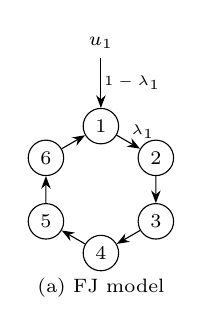
\begin{tikzpicture}[baseline=(c.base), scale=0.62]
        \foreach \i in {1,...,6} {
          \node[agent] (p\i) at ({90-60*(\i-1)}:1.3) {\i};
        }
        \node (c) at (0,0) {};
        \foreach \i/\j in {2/3,3/4,4/5,5/6,6/1} {
          \draw[edge] (p\i) -- (p\j);
        }
        \draw[edge] (p1) -- node[weight, above right] {$\lambda_1$} (p2);
        \draw[edge] (0,2.7) node[above, font=\scriptsize] {$u_1$}
          -- node[weight, right] {$1-\lambda_1$} (p1);
        \node at (0,-2.0) {\scriptsize (a) FJ model};
      \end{tikzpicture}
      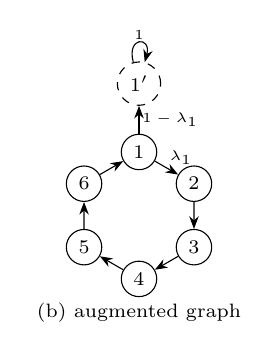
\begin{tikzpicture}[baseline=(c.base), scale=0.62]
        \foreach \i in {1,...,6} {
          \node[agent] (a\i) at ({90-60*(\i-1)}:1.3) {\i};
        }
        \node (c) at (0,0) {};
        \foreach \i/\j in {2/3,3/4,4/5,5/6,6/1} {
          \draw[edge] (a\i) -- (a\j);
        }
        \draw[edge] (a1) -- node[weight, above right] {$\lambda_1$} (a2);
        \node[agent, dashed, minimum size=5.5mm] (v1) at (0,2.7) {$1'$};
        \draw[edge] (a1) -- node[weight, right] {$1-\lambda_1$} (v1);
        \draw[selfloop] (v1) to node[weight, above] {$1$} (v1);
        \node at (0,-2.0) {\scriptsize (b) augmented graph};
      \end{tikzpicture}

      {\scriptsize Figure 4. Agent~$1$ the only prejudiced agent.}
  \end{columns}
  \vspace{1mm}
  \socially{A prejudice behaves as an extra agent that never changes its opinion, placed
  beside the prejudiced agent.}
  \detailbuttons{\go{bk-fj-consensus}{Consensus}\ \go{bk-augmented}{Augmented}}
\end{frame}

\begin{frame}[label=m-fj-centrality]{Influence centrality}
  \small
  \begin{itemize}
    \item The social power needs a consensus: in the FJ model it depends on $u$, and the
          augmented graph has $\geq n$ sinks.
    \item As in [5]: asymptotically stable, $u = x(0)$ (traditional FJ), so
          $x(\infty) = V x(0)$.
  \end{itemize}
  \begin{block}{Influence centrality [5]}
    \[ c = n^{-1} V^\top \mathbf{1}_n, \qquad
       \bar x = \tfrac1n \textstyle\sum_{i} x_i(\infty) = c^\top x(0) \]
    \footnotesize $c_i$: mean weight of $x_i(0)$ in the final opinions;
    $c \geq 0$, $c^\top\mathbf{1}_n = 1$, like $w$.
  \end{block}
  \begin{block}{Lemma 3.5 [5], in words}
    \footnotesize With $\Lambda = \alpha I$ and $W$ fully regular, $c_\alpha \to w$ as
    $\alpha \to 1^-$; for $\alpha = 0$, $V = I$ and $c_0 = \frac1n\mathbf{1}_n$.
  \end{block}
  \detailbuttons{\go{bk-centrality}{Lemma 3.5}}
\end{frame}

\begin{frame}[label=m-state-input]{Stubborn agent: state or input}
  \begin{columns}[T]
    \column{0.58\textwidth}
      \centering
      \only<1>{\includegraphics[width=\linewidth]{fj_stubborn_equivalence.eps}

      {\scriptsize Figure 6. Left: FDG with $A(1)$; right: FJ with $\lambda_1 = 0$,
      $u = x(0)$.}}%
      \only<2>{\includegraphics[width=\linewidth]{fj_stubborn_perturbation.eps}

      {\scriptsize Figure 7. Same models from $x_1(0) = 0.5$, $u$ unchanged.}}
    \column{0.40\textwidth}
      \footnotesize
      \only<1>{%
      \begin{itemize}
        \item Rewriting [5]: $\lambda_i = 0$, $u_i = x_i(0)$ for the stubborn agents,
              $\lambda_i = 1$ for the others.
        \item \alert{Same trajectories}, not the same stability: FDG never
              asymptotically stable (eigenvalue $1$), FJ asymptotically stable
              (Corollary~3.3).
      \end{itemize}}%
      \only<2>{%
      \begin{itemize}
        \item FDG: agent~$1$ keeps $0.5$, the group follows it: never forgotten.
        \item FJ: agent~$1$ back to $u_1 = 0$ after one step, same limit $Vu$.
        \item Stubborn row: $e_1^\top$ in $A(1)$, $0$ in $\Lambda W$: the eigenvalue
              $1$ becomes $0$.
      \end{itemize}}
      \vspace{1mm}
      \sociallycol{In the FDG model stubbornness is a memory in the state, never forgotten;
      in the FJ model it is an external input, and the state forgets $x(0)$.}
  \end{columns}
  \detailbuttons{\go{bk-state-input}{Spectra}\ \go{bk-rewritings}{Rewritings}}
\end{frame}

\begin{frame}[label=m-one-prej]{A single prejudice}
  \begin{columns}[T]
    \column{0.58\textwidth}
      \centering
      \includegraphics[width=\linewidth]{fj_one_prejudiced.eps}

      {\scriptsize Figure 9. Weight $1/2$ on agent~$1$. Left: FDG $A(1/2)$; right: FJ
      $1 - \lambda_1 = 1/2$.}
    \column{0.40\textwidth}
      \footnotesize
      \begin{itemize}
        \item All P-dependent: FJ \alert{asymptotically stable on a periodic network},
              with no self-loop.
        \item $V = \mathbf{1}_6 e_1^\top$: $x(\infty) = u_1\mathbf{1}_6 = 0$ for every
              $1 - \lambda_1 > 0$; FDG stops at $3/7$.
        \item $c = e_1$: one anchor takes \alert{all} the influence centrality, against
              $w_1 = 2/7$.
      \end{itemize}
      \vspace{1mm}
      \sociallycol{One anchored agent that influences everybody decides where the whole group
  ends, however weak its attachment.}
  \end{columns}
  \detailbuttons{\go{bk-one-prej}{Matrices}}
\end{frame}

\begin{frame}[label=m-all-prej]{Every agent prejudiced}
  \begin{columns}[T]
    \column{0.58\textwidth}
      \centering
      \includegraphics[width=\linewidth]{fj_all_prejudiced.eps}

      {\scriptsize Figure 10. Weight $0.2$ for all. Left: FDG $A = 0.2I + 0.8W$; right:
      FJ $\Lambda = 0.8I$, $u = x(0)$.}
    \column{0.40\textwidth}
      \footnotesize
      \begin{itemize}
        \item FDG: primitive, doubly stochastic: \alert{consensus} on the average $0.5$
              (Corollary~2.3).
        \item FJ: $V = 0.2\,(I - 0.8W)^{-1} > 0$: every prejudice in every final opinion,
              with different weights: \alert{disagreement}.
        \item Strongly connected: FDG never disagrees; the FJ disagreement comes from the
              prejudices.
      \end{itemize}
      \vspace{1mm}
      \sociallycol{Inertia gives way in the end, an anchor does not: different anchors keep the
  group divided, a cleavage of opinions [5].}
  \end{columns}
  \detailbuttons{\go{bk-all-prej}{Matrices}}
\end{frame}

\begin{frame}[label=m-aux]{Where no prejudice arrives}
  \only<1>{%
  \small
  Agents $1, 2, 3$ form a closed group, agents $4, 5, 6$ a chain that listens to it. One
  prejudiced agent, $\lambda = 0.5$. P-dependent agents shaded.

  \vspace{3mm}
  \centering
  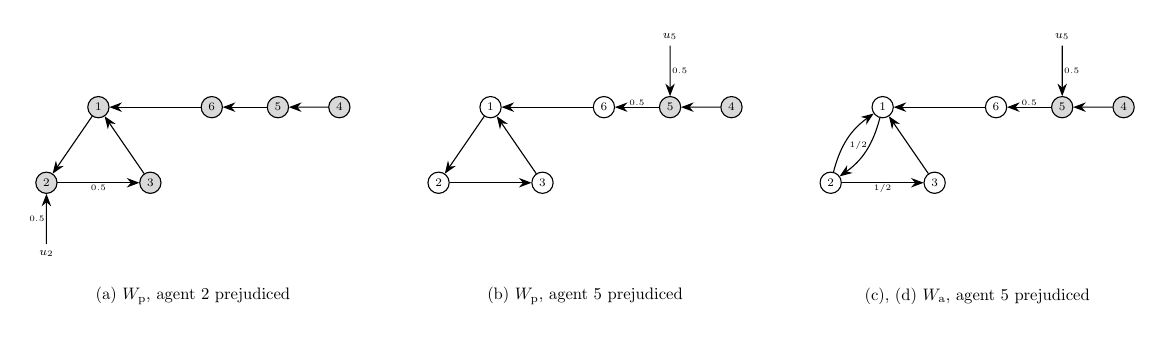
\begin{tikzpicture}[scale=0.6, every node/.append style={transform shape}, pdep/.style={agent, fill=gray!30}]
    \begin{scope}
      \node[pdep] (a1) at (0,1.1) {1}; \node[pdep] (a2) at (-1.1,-0.5) {2};
      \node[pdep] (a3) at (1.1,-0.5) {3}; \node[pdep] (a6) at (2.4,1.1) {6};
      \node[pdep] (a5) at (3.8,1.1) {5}; \node[pdep] (a4) at (5.1,1.1) {4};
      \draw[edge] (a1) -- (a2); \draw[edge] (a2) -- node[weight, below] {$0.5$} (a3); \draw[edge] (a3) -- (a1);
      \draw[edge] (a4) -- (a5); \draw[edge] (a5) -- (a6); \draw[edge] (a6) -- (a1);
      \draw[edge] (-1.1,-1.8) node[below, font=\scriptsize] {$u_2$} -- node[weight, left] {$0.5$} (a2);
      \node[font=\normalsize] at (2.0,-2.9) {(a) $W_{\mathrm{p}}$, agent~$2$ prejudiced};
    \end{scope}
    \begin{scope}[xshift=8.3cm]
      \node[agent] (a1) at (0,1.1) {1}; \node[agent] (a2) at (-1.1,-0.5) {2};
      \node[agent] (a3) at (1.1,-0.5) {3}; \node[agent] (a6) at (2.4,1.1) {6};
      \node[pdep] (a5) at (3.8,1.1) {5}; \node[pdep] (a4) at (5.1,1.1) {4};
      \draw[edge] (a1) -- (a2); \draw[edge] (a2) -- (a3); \draw[edge] (a3) -- (a1);
      \draw[edge] (a4) -- (a5); \draw[edge] (a5) -- node[weight, above] {$0.5$} (a6); \draw[edge] (a6) -- (a1);
      \draw[edge] (3.8,2.4) node[above, font=\scriptsize] {$u_5$} -- node[weight, right] {$0.5$} (a5);
      \node[font=\normalsize] at (2.0,-2.9) {(b) $W_{\mathrm{p}}$, agent~$5$ prejudiced};
    \end{scope}
    \begin{scope}[xshift=16.6cm]
      \node[agent] (a1) at (0,1.1) {1}; \node[agent] (a2) at (-1.1,-0.5) {2};
      \node[agent] (a3) at (1.1,-0.5) {3}; \node[agent] (a6) at (2.4,1.1) {6};
      \node[pdep] (a5) at (3.8,1.1) {5}; \node[pdep] (a4) at (5.1,1.1) {4};
      \draw[edge] (a1) to[bend left=20] (a2);
      \draw[edge] (a2) -- node[weight, below] {$1/2$} (a3); \draw[edge] (a3) -- (a1);
      \draw[edge] (a2) to[bend left=20] node[weight, below right] {$1/2$} (a1);
      \draw[edge] (a4) -- (a5); \draw[edge] (a5) -- node[weight, above] {$0.5$} (a6); \draw[edge] (a6) -- (a1);
      \draw[edge] (3.8,2.4) node[above, font=\scriptsize] {$u_5$} -- node[weight, right] {$0.5$} (a5);
      \node[font=\normalsize] at (2.0,-2.9) {(c), (d) $W_{\mathrm{a}}$, agent~$5$ prejudiced};
    \end{scope}
  \end{tikzpicture}

  \vspace{3mm}
  \raggedright
  {\small In $W_{\mathrm{p}}$ the closed group is a periodic cycle; in $W_{\mathrm{a}}$
  the edge $2 \to 1$ makes it aperiodic. In (d) only $x_2(0)$ moves, from $0.5$ to $1$.}

  \vspace{2mm}
  {\scriptsize Figure 11.}
  }%
  \only<2>{%
  \begin{columns}[T]
    \column{0.54\textwidth}
      \centering
      \includegraphics[width=\linewidth]{fj_auxiliary.eps}

      {\scriptsize Figure 12. $u = (0,\, 0.5,\, 1,\, 0.2,\, 0.9,\, 0.6)^\top$.}
    \column{0.44\textwidth}
      \footnotesize
      \begin{itemize}
        \item[(a)] Prejudice in the closed group: \alert{asymptotically stable}, all at
              $0.5$.
        \item[(b)] Outside, periodic closed group: $W^{22}$ not regular, \alert{no
              convergence}.
        \item[(c)] Aperiodic: \alert{convergent, not asymptotically stable}; $1,2,3,6$ at
              $0.4$, $4,5$ at $0.65$.
        \item[(d)] $x_2(0) = 1$: $0.6$ and $0.75$: the closed group \alert{remembers}.
      \end{itemize}
      \vspace{1mm}
      \sociallycol{Agents that no prejudice reaches form an FDG model of their own: they need
  aperiodicity and remember their initial opinions.}
  \end{columns}}
  \detailbuttons{\go{bk-aux}{Blocks}\ \go{bk-aux-table}{Table 2}}
\end{frame}

\begin{frame}[label=m-lemma]{Centrality meets social power}
  \begin{columns}[T]
    \column{0.58\textwidth}
      \centering
      \includegraphics[width=\linewidth]{fj_lemma24.eps}

      {\scriptsize Figure 13. $W = A(1/2)$, $\Lambda = \alpha I$, $u = x(0)$. Dashed:
      $w_1 = 2/7$, $w_2 = 1/7$.}
    \column{0.40\textwidth}
      \footnotesize
      \begin{itemize}
        \item $A(1/2)$ primitive, hence fully regular: Lemma~3.5 applies.
        \item $c_1$: from $1/6$ ($\alpha = 0$) to $w_1 = 2/7$; $c_2$ down to
              $w_2 = 1/7$.
        \item On the cycle $c_2$ first dips below $w_2$.
        \item Opening up to the others, the inertia of agent~$1$ counts more.
      \end{itemize}
      \vspace{1mm}
      \sociallycol{Social power: who leads a group that agrees. Influence centrality: who weighs
  most in a group that keeps disagreeing. The second becomes the first as the anchors are
  released.}
  \end{columns}
  \detailbuttons{\go{bk-lemma-numbers}{Numbers}}
\end{frame}

% ===========================================================================
\section{Conclusions}
% ===========================================================================

\begin{frame}[label=m-table]{FDG and FJ side by side}
  \centering
  \footnotesize
  \renewcommand{\arraystretch}{1.2}
  \begin{tabular}{@{}>{\raggedright\arraybackslash}p{2.9cm}
                  >{\raggedright\arraybackslash}p{4.9cm}
                  >{\raggedright\arraybackslash}p{5.2cm}@{}}
    \toprule
    & FDG model & FJ model \\
    \midrule
    Resistance & self-weight $a_{ii}$: inertia & attachment $1 - \lambda_i$: anchor \\
    Stubborn agent & $a_{ii} = 1$ (matrix only) & $\lambda_i = 0$, $u_i = x_i(0)$ (matrix
                                                   and input) \\
    Its opinion & a state & an input \\
    Asymptotic stability & never (eigenvalue $1$) & iff all agents P-dependent \\
    Strongly connected & consensus or no convergence & disagreement if the prejudices
                                                        that count differ \\
    Aperiodicity & always needed & only for P-independent agents \\
    Measure of power & social power $w$: needs consensus & influence centrality $c$: needs
                                                            $\rho(\Lambda W) < 1$,
                                                            $u = x(0)$ \\
    \bottomrule
  \end{tabular}

  \vspace{2mm}
  {\scriptsize Condensed from Table~3.}
  \detailbuttons{\go{bk-table}{Table 3}}
\end{frame}

\begin{frame}[label=m-messages]{Take-home messages}
  \begin{alertblock}{1.\ Inertia and anchor}
    \small A self-weight slows an agent down but lets it follow: one self-weight turns
    oscillations into consensus. A prejudice never gives way: one anchor decides where the
    group ends, different anchors keep it divided.
  \end{alertblock}
  \begin{alertblock}{2.\ State and input}
    \small The same stubborn opinion is a state in the FDG model (never asymptotically
    stable) and an input in the FJ model (asymptotically stable when the prejudices reach
    everybody). The augmented graph turns inputs back into states.
  \end{alertblock}
  \begin{alertblock}{3.\ Power}
    \small Social power grows gradually with the self-weight; one anchor takes all the
    influence centrality; with $\Lambda = \alpha I$ the influence centrality tends to the
    social power as $\alpha \to 1$.
  \end{alertblock}
\end{frame}

\begin{emptyframe}
  Thank you!
\end{emptyframe}

% ===========================================================================
% BACKUP SLIDES (not counted in the total; reached through the buttons)
% ===========================================================================
\appendix

\input{backup}

\end{document}
